\begin{filecontents*}[overwrite]{Note_refs.bib}
@article{aitken1997,
  author  = {Aitken, B. and Hanson, G. H. and Harrison, A. E.},
  title   = {Spillovers, Foreign Investment, and Export Behavior},
  journal = {Journal of International Economics},
  year    = {1997}, volume = {43}, number = {1--2}, pages = {103--132}}
@article{alfarourena2022,
  author  = {Alfaro-Ure{\~n}a, A. and Manelici, I. and Vasquez, J. P.},
  title   = {The Effects of Joining Multinational Supply Chains: New Evidence from Firm-to-Firm Linkages},
  journal = {Quarterly Journal of Economics},
  year    = {2022}, volume = {137}, number = {3}, pages = {1495--1552}}
@incollection{antras2014,
  author    = {Antr{\`a}s, P. and Yeaple, S. R.},
  title     = {Multinational Firms and the Structure of International Trade},
  booktitle = {Handbook of International Economics},
  editor    = {Gopinath, G. and Helpman, E. and Rogoff, K.},
  volume    = {4}, pages = {55--130}, publisher = {Elsevier}, address = {Amsterdam}, year = {2014}}
@article{bernard2018,
  author  = {Bernard, A. B. and Jensen, J. B. and Redding, S. J. and Schott, P. K.},
  title   = {Global Firms},
  journal = {Journal of Economic Literature},
  year    = {2018}, volume = {56}, number = {2}, pages = {565--619}}
@techreport{carballo2021,
  author      = {Carballo, J. and {Marra de Arti{\~n}ano}, I. and Ottaviano, G. I. P. and {Volpe Martincus}, C.},
  title       = {Linkages with Multinationals: The Effects on Domestic Firms' Exports},
  institution = {Inter-American Development Bank}, type = {Mimeo}, year = {2021}}
@article{carballo2026,
  author  = {Carballo, J. and {Marra de Arti{\~n}ano}, I. and {Volpe Martincus}, C.},
  title   = {The Impact of Investment Promotion on Multinational Production: Firm-Level Evidence},
  journal = {Journal of Development Economics},
  year    = {2026}, volume = {180}, pages = {103666}}
@article{chaney2008,
  author  = {Chaney, T.},
  title   = {Distorted Gravity: The Intensive and Extensive Margins of International Trade},
  journal = {American Economic Review},
  year    = {2008}, volume = {98}, number = {4}, pages = {1707--1721}}
@article{clapp2015,
  author  = {Clapp, J.},
  title   = {{ABCD} and Beyond: From Grain Merchants to Agricultural Value Chain Managers},
  journal = {Canadian Food Studies},
  year    = {2015}, volume = {2}, number = {2}, pages = {126--135}}
@article{conconi2016,
  author  = {Conconi, P. and Sapir, A. and Zanardi, M.},
  title   = {The Internationalization Process of Firms: From Exports to {FDI}},
  journal = {Journal of International Economics},
  year    = {2016}, volume = {99}, pages = {16--30}}
@article{damgaard2024,
  author  = {Damgaard, J. and Elkjaer, T. and Johannesen, N.},
  title   = {What Is Real and What Is Not in the Global {FDI} Network?},
  journal = {Journal of International Money and Finance},
  year    = {2024}, volume = {140}, pages = {102971}}
@article{ekholm2007,
  author  = {Ekholm, K. and Forslid, R. and Markusen, J. R.},
  title   = {Export-Platform Foreign Direct Investment},
  journal = {Journal of the European Economic Association},
  year    = {2007}, volume = {5}, number = {4}, pages = {776--795}}
@article{freund2015,
  author  = {Freund, C. and Pierola, M. D.},
  title   = {Export Superstars},
  journal = {Review of Economics and Statistics},
  year    = {2015}, volume = {97}, number = {5}, pages = {1023--1032}}
@article{harding2011,
  author  = {Harding, T. and Javorcik, B. S.},
  title   = {Roll Out the Red Carpet and They Will Come: Investment Promotion and {FDI} Inflows},
  journal = {Economic Journal},
  year    = {2011}, volume = {121}, number = {557}, pages = {1445--1476}}
@incollection{head2014,
  author    = {Head, K. and Mayer, T.},
  title     = {Gravity Equations: Workhorse, Toolkit, and Cookbook},
  booktitle = {Handbook of International Economics},
  editor    = {Gopinath, G. and Helpman, E. and Rogoff, K.},
  volume    = {4}, pages = {131--195}, publisher = {Elsevier}, address = {Amsterdam}, year = {2014}}
@article{helpman2004,
  author  = {Helpman, E. and Melitz, M. J. and Yeaple, S. R.},
  title   = {Export versus {FDI} with Heterogeneous Firms},
  journal = {American Economic Review},
  year    = {2004}, volume = {94}, number = {1}, pages = {300--316}}
@article{javorcik2004,
  author  = {Javorcik, B. S.},
  title   = {Does Foreign Direct Investment Increase the Productivity of Domestic Firms? In Search of Spillovers through Backward Linkages},
  journal = {American Economic Review},
  year    = {2004}, volume = {94}, number = {3}, pages = {605--627}}
@article{keller2013,
  author  = {Keller, W. and Yeaple, S. R.},
  title   = {The Gravity of Knowledge},
  journal = {American Economic Review},
  year    = {2013}, volume = {103}, number = {4}, pages = {1414--1444}}
@article{kandel2008,
  author  = {Kandel, W.},
  title   = {Hired Farmworkers a Major Input for Some {U.S.} Farm Sectors},
  journal = {Amber Waves},
  year    = {2008},
  note    = {April 2008. Washington, DC: US Department of Agriculture, Economic Research Service}}
@article{mayneris2015,
  author  = {Mayneris, F. and Poncet, S.},
  title   = {{Chinese} Firms' Entry to Export Markets: The Role of Foreign Export Spillovers},
  journal = {World Bank Economic Review},
  year    = {2015}, volume = {29}, number = {1}, pages = {150--179}}
@techreport{murphy2012,
  author      = {Murphy, S. and Burch, D. and Clapp, J.},
  title       = {Cereal Secrets: The World's Largest Grain Traders and Global Agriculture},
  institution = {Oxfam International}, type = {Oxfam Research Reports}, address = {Oxford}, year = {2012}}
@article{ramondo2016,
  author  = {Ramondo, N. and Rappoport, V. and Ruhl, K. J.},
  title   = {Intrafirm Trade and Vertical Fragmentation in {U.S.} Multinational Corporations},
  journal = {Journal of International Economics},
  year    = {2016}, volume = {98}, pages = {51--59}}
@article{rauch1999,
  author  = {Rauch, J. E.},
  title   = {Networks versus Markets in International Trade},
  journal = {Journal of International Economics},
  year    = {1999}, volume = {48}, number = {1}, pages = {7--35}}
@article{reardon2009,
  author  = {Reardon, T. and Barrett, C. B. and Berdegu{\'e}, J. A. and Swinnen, J. F. M.},
  title   = {Agrifood Industry Transformation and Small Farmers in Developing Countries},
  journal = {World Development},
  year    = {2009}, volume = {37}, number = {11}, pages = {1717--1727}}
@article{swinnen2007,
  author  = {Swinnen, J. F. M. and Maertens, M.},
  title   = {Globalization, Privatization, and Vertical Coordination in Food Value Chains in Developing and Transition Countries},
  journal = {Agricultural Economics},
  year    = {2007}, volume = {37}, number = {s1}, pages = {89--102}}
@article{torslov2023,
  author  = {T{\o}rsl{\o}v, T. and Wier, L. and Zucman, G.},
  title   = {The Missing Profits of Nations},
  journal = {Review of Economic Studies},
  year    = {2023}, volume = {90}, number = {3}, pages = {1499--1534}}
@misc{trase2020,
  author       = {{Trase}},
  title        = {{Argentina} Crushing Capacity Drives Up Imported Soy Deforestation Risk in 2018},
  howpublished = {Trase Insights}, note = {1 July 2020}, year = {2020}}
@book{unctad2009,
  author    = {{UNCTAD}},
  title     = {{World Investment Report 2009}: Transnational Corporations, Agricultural Production and Development},
  publisher = {United Nations}, address = {New York and Geneva}, year = {2009}}
@book{unctad2013,
  author    = {{UNCTAD}},
  title     = {{World Investment Report 2013}: Global Value Chains: Investment and Trade for Development},
  publisher = {United Nations}, address = {New York and Geneva}, year = {2013}}
@article{volpe2008,
  author  = {{Volpe Martincus}, C. and Carballo, J.},
  title   = {Is Export Promotion Effective in Developing Countries? Firm-Level Evidence on the Intensive and the Extensive Margins of Exports},
  journal = {Journal of International Economics},
  year    = {2008}, volume = {76}, number = {1}, pages = {89--106}}
@book{volpe2021,
  author    = {{Volpe Martincus}, C. and {Marra de Arti{\~n}ano}, I. and Sztajerowska, M. and Carballo, J.},
  title     = {Making the Invisible Visible: Investment Promotion and Multinational Production in {Latin America} and the {Caribbean}},
  publisher = {Inter-American Development Bank}, address = {Washington, DC}, year = {2021}}
\end{filecontents*}
\documentclass[article, 12pt, 3p]{elsarticle}

\usepackage{natbib} 
\setcitestyle{authoryear,open={(},close={)}}
%\bibliographystyle{plainnat}

\usepackage{etoolbox,comment,setspace,fancyhdr,hyperref,color,graphicx,subcaption,booktabs,rotating,multirow}

\captionsetup[subfigure]{labelformat=simple,labelsep=space}
\renewcommand\thesubfigure{(\roman{subfigure})}

\newcounter{rowfig}
\renewcommand{\therowfig}{\Alph{rowfig}}

\usepackage{amsmath,amsthm,amssymb,amstext,bbold,amsfonts}
\usepackage{float,caption}
\usepackage{threeparttable}
\usepackage{lscape}
\usepackage{bbm}
\usepackage{adjustbox}
\usepackage[tracking=true]{microtype}
%\usepackage[pdftex, letterpaper, margin=1in, headheight=-.25cm]{geometry}
 %\usepackage[abbr]{harvard}
 
\hypersetup{
  colorlinks   = true, %Colours links instead of ug dly boxes
  urlcolor     = blue, %Colour for external hyperlinks
  linkcolor    = black, %Colour of internal links 
  citecolor   = blue %Colour of citations
}

\newtheorem{proposition}{Proposition}
\newtheorem{definition}{Definition}
\newtheorem{assumption}{Assumption}
\newtheorem{condition}{Condition}
\newtheorem{lemma}{Lemma}
\newtheorem{conjecture}{Conjecture}
\newtheorem{corollary}{Corollary}
\numberwithin{corollary}{proposition}
%\numberwithin{equation}{section}
% [[prompt01]] original: \numberwithin{equation}{}

%\newcommand{\inv}{\makebox[0pt][l]{$^{-1}$}}
\pdfoptionpdfminorversion=6 

%Define argmax
\DeclareMathOperator*{\argmax}{arg\,max}

%%Put space between captions and figures.
%\setlength{\belowcaptionskip}{6pt}

\makeatletter
\def\ps@pprintTitle{%
   \let\@oddhead\@empty
   \let\@evenhead\@empty
   \let\@oddfoot\@empty
   \let\@evenfoot\@oddfoot
}
\makeatother
\usepackage{ragged2e}
\usepackage{setspace} 
\usepackage{caption}
 \usepackage[space]{grffile} % For spaces in paths
 \makeatletter % For spaces in paths
 \patchcmd\Gread@eps{\@inputcheck#1 }{\@inputcheck"#1"\relax}{}{}
 \makeatother
\usepackage[utf8]{inputenc}
% [[prompt01]] original: \usepackage{stackrel}
\IfFileExists{stackrel.sty}{\usepackage{stackrel}}{}
\usepackage{array}
\usepackage{siunitx}
\usepackage{makecell}
\newcolumntype{N}[1]{>{\centering\arraybackslash}p{#1}}
\newcolumntype{L}[1]{>{\raggedright\arraybackslash}p{#1}}
\newlength{\labelw}\setlength{\labelw}{0.22\textwidth}
\newlength{\labelwwide}\setlength{\labelwwide}{0.36\textwidth}
\newlength{\labelwnarrow}\setlength{\labelwnarrow}{0.19\textwidth}
\newcommand{\colwfor}[2]{\dimexpr(\textwidth-(#2)-\tabcolsep*\numexpr2*#1+2\relax)/#1\relax}
\newcommand{\colwform}[3]{\dimexpr(\textwidth-(#3)-\tabcolsep*\numexpr2*#1+2*#2\relax)/#1\relax}
\newcommand{\colw}{\colwfor{6}{\labelw}}
\newcommand{\colwvii}{\colwfor{7}{\labelw}}
\newcommand{\colwnarrow}{\colwfor{8}{\labelw}}
\newcommand{\notesize}{\footnotesize}
\setlength{\extrarowheight}{4pt}
\renewcommand\normalsize{\fontsize{11}{8}\selectfont}
\newcommand\narrowstyle{\SetTracking{encoding=*}{-10}\lsstyle}
\newcommand\vnarrowstyle{\SetTracking{encoding=*}{-40}\lsstyle}
\newcommand\vvnarrowstyle{\SetTracking{encoding=*}{-75}\lsstyle}

\newcommand\narrowtext[1]{\textls[-10]{#1}}
\newcommand\vnarrowtext[1]{\textls[-40]{#1}}
\newcommand\vvnarrowtext[1]{\textls[-75]{#1}}

\makeatletter
\renewcommand\footnotesize{%
   \@setfontsize\footnotesize\@ixpt{9}%
   \abovedisplayskip 8\p@ \@plus2\p@ \@minus4\p@
   \abovedisplayshortskip \z@ \@plus\p@
   \belowdisplayshortskip 4\p@ \@plus2\p@ \@minus2\p@
   \def\@listi{\leftmargin\leftmargini
               \topsep 4\p@ \@plus2\p@ \@minus2\p@
               \parsep 2\p@ \@plus\p@ \@minus\p@
               \itemsep \parsep}%
   \belowdisplayskip \abovedisplayskip
}
\makeatother

\usepackage{setspace}
\usepackage[T1]{fontenc}
\usepackage{array}
\usepackage{longtable}
\usepackage{pdfpages}
\usepackage{dsfont}
\newcommand{\bc}{\begin{center}}
\newcommand{\ec}{\end{center}}
\newcommand{\bt}{\begin{tabular}}
\newcommand{\et}{\end{tabular}}
\newcommand{\bi}{\begin{itemize}}
\newcommand{\ei}{\end{itemize}}
\newcommand{\ben}{\begin{enumerate}}
\newcommand{\een}{\end{enumerate}}
\newcommand{\bd}{\begin{displaymath}}
\newcommand{\ed}{\end{displaymath}}
\newcommand{\beann}{\begin{eqnarray*}}
\newcommand{\eeann}{\end{eqnarray*}}
\newcommand{\bea}{\begin{eqnarray}}
\newcommand{\eea}{\end{eqnarray}}
\newcommand{\ba}{\begin{array}}
\newcommand{\ea}{\end{array}}
\newcommand{\bma}{\begin{pmatrix}}
\newcommand{\ema}{\end{pmatrix}}
%}}}
%Math Shortcuts {{{
\newcommand{\Ra}{\Rightarrow}
\newcommand{\bbR}{\mathbb{R}}
\newcommand{\bbY}{\mathbb{Y}}
\newcommand{\bbF}{\mathbb{F}}
\newcommand{\bbS}{\mathbb{S}}
\newcommand{\bbN}{\mathbb{N}}
\newcommand{\bbG}{\mathbb{G}}
\newcommand{\bbT}{\mathbb{T}}
\newcommand{\deB}{\mathcal{B}}
\newcommand{\deW}{\mathcal{W}}
\newcommand{\deR}{\mathcal{R}}
\newcommand{\deF}{\mathcal{F}}
\newcommand{\deA}{\mathcal{A}}
\newcommand{\deY}{\mathcal{Y}}
\newcommand{\deS}{\mathcal{S}}
\newcommand{\deL}{\mathcal{L}}
\newcommand{\deH}{\mathcal{H}}
\newcommand{\deE}{\mathcal{E}}
\newcommand{\deP}{\mathcal{P}}
\newcommand{\deG}{\mathcal{G}}
\newcommand{\deT}{\mathcal{T}}
\newcommand{\deff}{\mathcal{f}}
\newcommand{\dep}{\mathcal{p}}
\newcommand{\E}{\mathnormal{E}}
\newcommand{\var}{\mathnormal{V\!AR}}
\newcommand{\Cov}{\mathnormal{COV}}
\newcommand{\Corr}{\mathnormal{CORR}}
\newcommand{\Prob}{\mathnormal{Prob}}
%}}}
%Additional Shortcuts {{{
\newcommand{\mD}{\displaystyle}
\newcommand{\mT}{\textstyle}
\newcommand{\mS}{\scriptstyle}
\newcommand{\mSS}{\scriptscriptstyle}
\newcommand{\m}[1]{\,#1\,}
\newcommand{\nn}{\nonumber}
\newcommand{\colorEmphText}{\color{blue}}
\newcommand{\colorEmphBackground}{\color{yellow}}
%}}}
% \usepackage[stable]{footmisc} 
\newcommand*{\mycommand}[1]{\texttt{\emph{#1}}}
% [[prompt01]] original: \renewcommand*{\thefootnote}{\fnsymbol{footnote}}
%% these three are essential for estout
\usepackage{booktabs}  % neatly formatting lines
\usepackage{threeparttable}    
\usepackage{dcolumn}    % aligning decimals
    \newcolumntype{d}[1]{D{.}{.}{#1}}
% Estout LaTeX wrapper (by Jörg Weber)
\let\estinput=\input % define a new input command so that we can still flatten the document
\newcommand{\estwide}[3]{
		\vspace{.75ex}{
			%\textsymbols% Note the added command here
			\begin{tabular*}
			{\textwidth}{@{\hskip\tabcolsep\extracolsep\fill}l*{#2}{#3}}
			\toprule
			\estinput{#1}
			\addlinespace[.75ex]
			\end{tabular*}
			}
		}	
\newcommand{\estauto}[3]{
		\vspace{.75ex}{
			%\textsymbols% Note the added command here
			\begin{tabular}{l*{#2}{#3}}
			\toprule
			\estinput{#1}
			\\ \bottomrule           % 08 Dec 2021. Add these slashes.
			\addlinespace[-.75]
			\end{tabular}
			}
		}
% Allow line breaks with \\ in specialcells
\newcommand{\specialcell}[2][c]{%
    \begin{tabular}[#1]{@{}c@{}}#2\end{tabular}
}
\usepackage{float}
\usepackage[section]{placeins}
% [[prompt02d]] floats share pages with text instead of going to float pages
\renewcommand{\topfraction}{0.9}
\renewcommand{\bottomfraction}{0.8}
\renewcommand{\textfraction}{0.07}
\renewcommand{\floatpagefraction}{0.85}
\setcounter{topnumber}{3}
\setcounter{bottomnumber}{2}
\setcounter{totalnumber}{4}
\setlength{\floatsep}{10pt plus 2pt minus 2pt}
\setlength{\textfloatsep}{14pt plus 2pt minus 2pt}
\setlength{\intextsep}{12pt plus 2pt minus 2pt}
\newcommand{\sym}[1]{\rlap{#1}}% Thanks David Carlisle
\usepackage{hhline}
\captionsetup{font=normalsize} 


 % Note/Source/Text after Tables
\newcommand{\figtext}[1]{
	\vspace{-1.9ex}
	\captionsetup{justification=justified,font=scriptsize}
	\caption*{\hspace{6pt}\hangindent=1.5em #1}
	} 
\newcommand{\fignote}[1]{\figtext{\emph{Note:~}~#1}}

\newcommand{\figsource}[1]{\figtext{\emph{Source:~}~#1}}

% Add significance note with \starnote
\newcommand{\starnote}{\figtext{* p < 0.1, ** p < 0.05, *** p < 0.01. Standard errors in parentheses.}}
% [[prompt01]] added: source note of every table and figure (wording from main.tex l. 16)
% [[prompt02]] original: \newcommand{\srcnote}{\textit{Source:} Authors' calculations based on customs data matched to Orbis and Dun \& Bradstreet.}
\newcommand{\srcnote}{\textit{Source:} Authors' calculations based on customs data matched to Orbis (Bureau van Dijk) and Dun \& Bradstreet.}
%\usepackage{etoolbox} % to hook into `figure` and reset the mysubfig counter

% [[prompt01]] original: \usepackage{subfig}


% Checkmarks
\usepackage{tikz}
\newcommand{\tikzxmark}{%
\tikz[scale=0.23] {
    \draw[line width=0.7,line cap=round] (0,0) to [bend left=6] (1,1);
    \draw[line width=0.7,line cap=round] (0.2,0.95) to [bend right=3] (0.8,0.05);
}}
\newcommand{\tikzcmark}{% 
\tikz[scale=0.23] {
    \draw[line width=0.7,line cap=round] (0.25,0) to [bend left=10] (1,1);
    \draw[line width=0.8,line cap=round] (0,0.35) to [bend right=1] (0.23,0);
}}
%\renewcommand{\arraystretch}{0.9}
 \makeatletter
\newcommand*\mysize{%
  \@setfontsize\mysize{7.5}{9.0}%
}

\makeatother
% For reference:
%\[
%    \checkmark
%    \tikzxmark
%    \tikzcmark
%\]

%\onehalfspacing

\begin{document}

\title{$\,$\\ $\,$\\ $\,$\\\vspace{-4.9em}\LARGE\textbf{Multinational Firms and Agricultural Trade in Latin America}\footnote{The views and interpretations in this paper are strictly those of the authors and should not be attributed to the Inter-American Development Bank, its executive directors, or its member countries.}}
\author{\vskip 2em This version: October 2026\\[2pt] \small Preliminary draft, please do not circulate}

\thispagestyle{empty}
\maketitle
\setcounter{page}{0}\setcounter{footnote}{0}
\renewcommand\normalsize{\fontsize{12}{20}\selectfont}\normalsize
\newpage

%======================================================================
\section{Introduction}\label{sec:intro}
%======================================================================
Multinational firms are at the center of international trade. About 80 percent of world trade is linked to
their international production networks \citep{unctad2013}. In a sample of 32 countries, the largest exporter
accounts for about 14 percent of non-oil exports and the five largest for about 30 percent \citep{freund2015}. Agriculture is no exception. Four trading companies, the ABCD, control over 70 percent of the
global grain market \citep{murphy2012,clapp2015}. Multinational firms from developed countries
lead the supplier, processing, trading and retail stages of agricultural value chains \citep{unctad2009}.

Agriculture makes up 35 percent of the merchandise exports of the nine Latin American countries in this study,
and more than half in Argentina, Paraguay and Uruguay. Little is known about who ships these exports. Customs
records do not say who owns the exporting firm, and statistics on foreign direct investment do not say which firms
export which products to which markets.

This paper measures how much of Latin America's agricultural exports multinational firms ship, where their
parents are based, how concentrated their ownership is, and whether exports are larger and distance a smaller
barrier where they are present.

A new database links the customs records of all the exports of nine countries over 2012--2018 to ownership
data from Orbis and Dun \& Bradstreet. The countries are Argentina, Chile, Colombia, Costa Rica, the
Dominican Republic, El Salvador, Paraguay, Peru and Uruguay. The database classifies every exporter as a foreign
multinational, a domestic multinational or a local firm.

The results are six stylized facts. First, multinational firms ship almost half of agricultural exports: 47.5
percent in 2018, 39.6 percent through foreign affiliates and 7.9 percent through domestic ones, and between 47 and 50
percent in every year of 2012--2018. Second, the parents of foreign affiliates are based in a few countries. The
United States accounts for 24 percent of their exports, the Netherlands for 12 percent and groups whose parent is
recorded in Switzerland, Liechtenstein and other investment hubs for 26 percent. Third, large groups dominate: groups with
more than 100 affiliates worldwide are 15 percent of all parents but ship half of the exports of foreign affiliates.
Fourth, product--destination pairs with more multinational firms export more, and so do local firms there. Fifth, this association is stronger for field crops, such as cereals and oilseeds, than for horticultural
crops. Sixth, the distance elasticity of exports is smaller for multinational affiliates than for local firms, by about 15 percent, and by about 40 percent when the group has an affiliate in the destination or the destination is the parent's country. These regression estimates are conditional correlations.

The paper adds to three literatures. Work on firms in trade, mostly on manufacturing in high-income countries,
studies why some become multinationals and a few account for most trade \citep[see, e.g.,][]{helpman2004,antras2014,bernard2018,ramondo2016}; the paper covers all
agricultural exporters of nine countries. Work on agricultural value chains focuses on specific chains
or companies \citep{swinnen2007,reardon2009,unctad2009,murphy2012,clapp2015}; we measure the multinational share of all agricultural exports. Work on foreign investment studies its links
with host-country firms \citep{javorcik2004,alfarourena2022}. Firms are more likely to export
when multinational exporters are nearby \citep{aitken1997}, when nearby foreign firms serve the market
\citep{mayneris2015} or after they start selling to a multinational \citep{carballo2021}. Our local-firm results are in line with this evidence. Trade falls with distance \citep{head2014}, through fixed costs \citep{chaney2008} and search costs \citep{rauch1999}; affiliate sales also fall with distance from the parent \citep{keller2013}, and firms often export to a market before investing there \citep{conconi2016}. We compare the distance elasticity of affiliates and local firms.

The results bear on investment promotion, which attracts multinational firms \citep{harding2011,volpe2021,carballo2026}. They also show that the recorded parent of a sizable share of foreign-affiliate exports sits in an investment hub, a pattern documented for foreign direct investment and corporate profits at large \citep{damgaard2024,torslov2023}.

Section~\ref{sec:data} describes the data, Section~\ref{sec:results} presents the six stylized facts and
Section~\ref{sec:concl} concludes.\footnote{The Appendix reports descriptive statistics on the composition of agricultural exports by year, destination, product and type of exporter.}

%======================================================================
\section{Data}\label{sec:data}
%======================================================================
The data come from two sources. The first is the export transactions recorded by the customs agencies of the
nine countries. For each export, they report the tax identifier and name of the exporting firm, the product at the
six-digit level of the Harmonized System (2007 revision), the destination, the year and the value in US dollars
(FOB). The period is 2012--2018, the years in which all nine countries are observed, and agricultural products are
chapters 01 to 24 of the Harmonized System.

The second source is ownership data from Orbis, compiled by Bureau van Dijk, and the 2025 release of Dun \&
Bradstreet. Orbis reports each company's global ultimate owner, defined with ownership thresholds of 25 and 50
percent, the country of the company and of its owner, and up to three national identifiers. It links about 17
million companies to about 13 million ultimate owners. Dun \& Bradstreet reports the name and country of each
company's global ultimate parent. The two are combined into one file by matching company names, with an artificial
intelligence agent reviewing each candidate pair.

Exporters are linked to this file in three stages, each applied to the exporters left unmatched by the previous
one. The first matches tax identifiers. The second matches names, within each country and then across countries,
by the TF-IDF cosine similarity of three-character sequences. It keeps pairs with a similarity of at least 0.6 that
a large language model confirms as the same company or group. The third is a manual review of the 500 largest
unmatched exporters in each country. Missing parent countries of matched firms are recovered from the raw ownership
links in Orbis and a further review with the language model. The country of the parent is known for 89 percent of
the agricultural exports of foreign affiliates.

Exporters linked to the file are classified as affiliates of multinational firms (MNEs). An
affiliate is a \emph{domestic} MNE when its ultimate parent is located in the exporting country
and a \emph{foreign} MNE otherwise; matched exporters without a recorded parent country are treated
as foreign. Exporters that cannot be linked to the file are \emph{local} firms, which we also refer
to as non-MNE firms. Since the match relies on ownership links, the head company of a group that
exports from its own country cannot be identified and is counted as a local firm.

The sample is described with the data for 2018, the last year in which the nine countries are observed. The
composition of agricultural exports and the role of multinational firms change little between 2012 and 2018, so a
single year shows the main features of the period.\footnote{Appendix Tables~\ref{tab:ap_trend} and~\ref{tab:ap_cy} report exports by type of exporter and the multinational share by exporting country in each year, and Appendix Tables~\ref{tab:ap_summary}, \ref{tab:ap_sample} and~\ref{tab:ap_desttab} report the sample summary and exports by exporting country and by destination region as annual averages over 2012--2018.}

In 2018, 12,993 firms exported 875 agricultural products to 211 countries, for a total of US\$78.5 billion
(Table~\ref{tab:summary}). Destinations are the countries with an ISO3 code, so shipments to free trade zones and
to the exporting country itself do not add destinations.
% ---- Table: Agricultural sample summary, 2018
\begin{table}[htbp]
\centering
\caption{Agricultural sample summary, 2018}
\label{tab:summary}
{\small\setlength{\tabcolsep}{4pt}\setlength{\extrarowheight}{1pt}
\input{tables/agro2018/tab_agp_summary_general_fx3}}

\begin{minipage}{0.95\linewidth}
\notesize
\vspace{0.6em}
\textit{Notes:} Agricultural exports (HS 01--24) of the nine countries in 2018. Destination countries: distinct ISO3 codes of the importing countries; free trade zones and shipments to the exporting country itself are not counted.\\
\srcnote
\end{minipage}
\end{table}

Agriculture accounts for 35 percent of the merchandise exports of the nine countries, with wide differences
across them (Table~\ref{tab:sample}). Its weight is 84 percent in Paraguay, 56 percent in Argentina and 52 percent
in Uruguay, and between 17 and 24 percent in Colombia, El Salvador, Peru, the Dominican Republic and Chile.
Argentina alone ships 44 percent of the region's agricultural exports.
% ---- Table: Agricultural exports, by exporting country, 2018
\begin{table}[htbp]
\centering
\caption{Agricultural exports, by exporting country, 2018}
\label{tab:sample}
{\small\setlength{\tabcolsep}{4pt}\setlength{\extrarowheight}{1pt}
\input{tables/agro2018/tab_agp_sample_nomne_fx2}}

\begin{minipage}{0.95\linewidth}
\notesize
\vspace{0.6em}
\textit{Notes:} Agricultural exports (HS 01--24) in 2018. Exporters are distinct tax identifiers within each country. Destinations are counted as in Table~\ref{tab:summary}. Exports in US\$ billion. Agriculture in total exports: percent of the country's merchandise exports.\\
\srcnote
\end{minipage}
\end{table}

%======================================================================
\section{Stylized facts}\label{sec:results}
%======================================================================
This section presents six stylized facts. The first three describe who owns the agricultural exports of the
nine countries in 2018. The last three relate multinational presence to export performance in regressions on
2012--2018. Since the data do not provide variation in multinational presence unrelated to exports, we interpret
these estimates as correlations rather than causal effects.

\subsection{Fact 1: Multinationals ship almost half of agricultural exports}\label{sec:owners}

Multinational firms shipped 47.5 percent of the agricultural exports of the nine countries in 2018, 39.6 percent
through foreign affiliates and 7.9 percent through domestic ones (Figure~\ref{fig:f1}, Panel A). These exports come
from 3,181 affiliates of 1,908 multinational groups, whose parents are based in 112 countries, while local firms ship
the remaining 52.5 percent (Table~\ref{tab:mne}). The share is highest in Uruguay (72 percent) and Paraguay (69
percent), two of the countries where agriculture weighs most in exports, and lowest in El Salvador (30 percent),
Colombia (40 percent) and Peru (40 percent). Foreign affiliates ship more than domestic ones in every country; the
gap is smallest in Chile (30 against 19 percent) and Colombia (27 against 13 percent), where domestic groups are
larger.
% ---- Table: Multinational firms in agricultural exports, 2018
\begin{table}[htbp]
\centering
\caption{Multinational firms in agricultural exports, 2018}
\label{tab:mne}
{\small\setlength{\tabcolsep}{4pt}\setlength{\extrarowheight}{1pt}
\input{tables/agro2018/tab_agp_summary_mne_fx3}}

\begin{minipage}{0.95\linewidth}
\notesize
\vspace{0.6em}
\textit{Notes:} Agricultural exports (HS 01--24) of the nine countries in 2018. Multinational affiliates: exporters linked to Orbis or Dun \& Bradstreet. Shares by type of exporter are percent of agricultural export value.\\
\srcnote
\end{minipage}
\end{table}

% ---- Figure: Multinational share of agricultural exports, by exporting country, 2018
\begin{figure}[htbp]
\centering
\caption{Multinational share of agricultural exports, by exporting country, 2018}
\label{fig:f1}
{\small\textit{Panel A. Foreign and domestic multinationals}}\par\vspace{1pt}
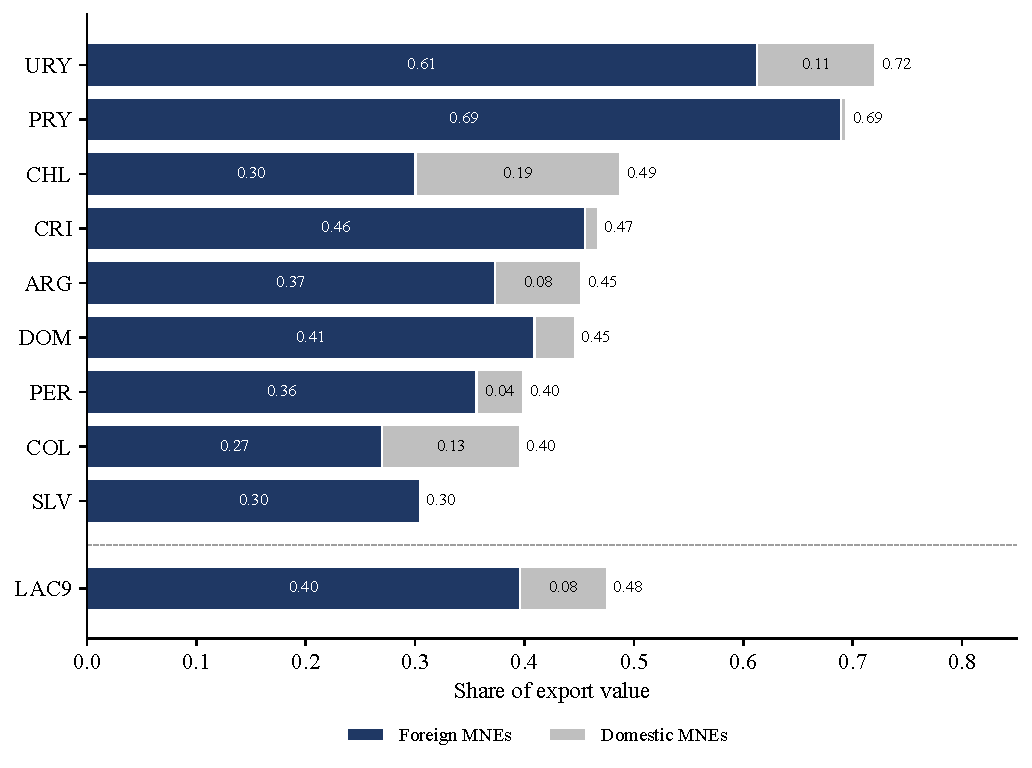
\includegraphics[width=0.72\textwidth,height=0.30\textheight,keepaspectratio]{figures/agro2018/fig_agp_origin_lac9.pdf}
\par\vspace{3pt}
{\small\textit{Panel B. Multinationals by parent country}}\par\vspace{1pt}
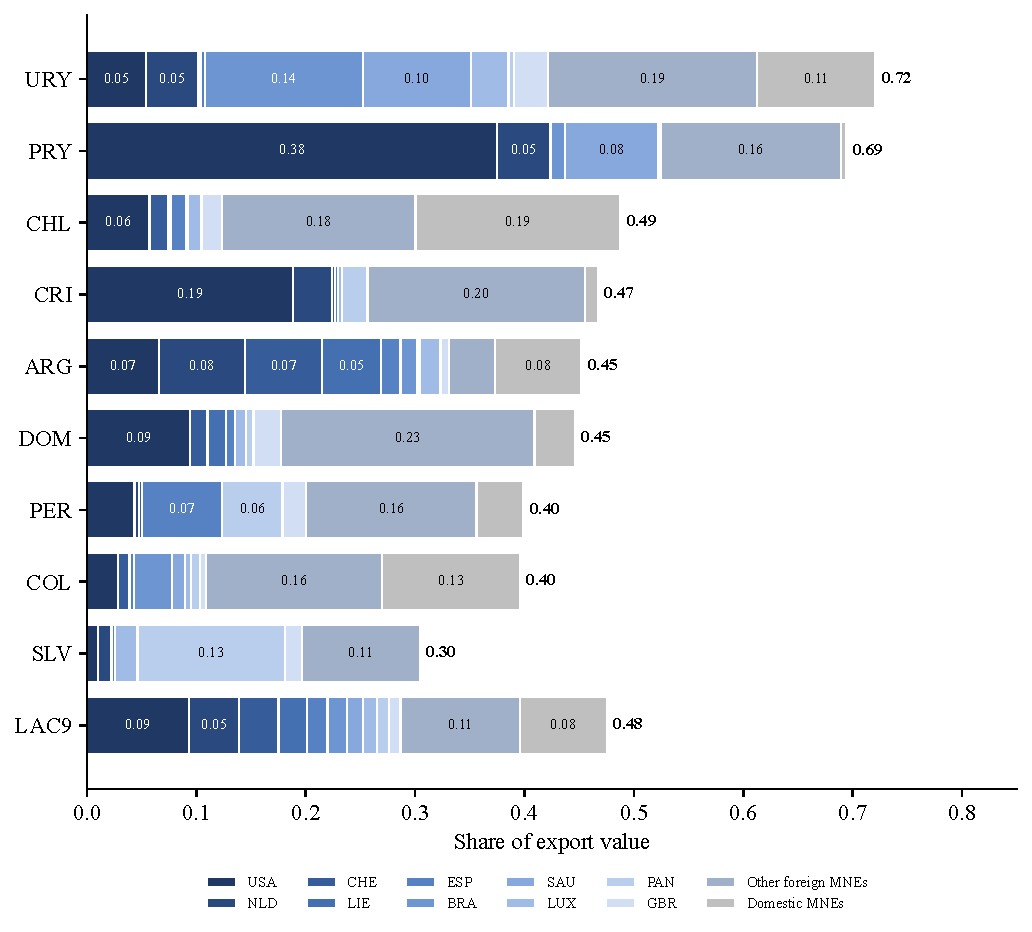
\includegraphics[width=0.85\textwidth,height=0.32\textheight,keepaspectratio]{figures/agro2018/fig_wp1a_origin_by_parent_lac9.pdf}

\begin{minipage}{0.9\linewidth}
\notesize
\vspace{0.6em}
\textit{Notes:} Shares of agricultural export value (HS 01--24) in 2018. Panel A: LAC9 is the nine countries together; the number at the end of each bar is the total MNE share. Panel B: LAC9 at the bottom; the foreign share split among the ten largest parent countries and all other foreign parents (including matched firms with no recorded parent country); domestic MNEs have their parent in the exporting country.\\
\srcnote
\end{minipage}
\end{figure}

The parents behind these shares differ across countries (Figure~\ref{fig:f1}, Panel B). In Paraguay, groups based
in the United States ship 38 percent of the country's agricultural exports, and in Costa Rica 19 percent. In
Argentina, foreign ownership is spread among Dutch (8 percent), Swiss (7 percent), US (7 percent) and Liechtenstein
(6 percent) groups. Brazilian and Saudi groups ship 14 and 10 percent of the agricultural exports of Uruguay, Spanish
groups 7 percent of those of Peru, and groups based in Panama 14 percent of those of El Salvador.

\FloatBarrier
\subsection{Fact 2: Parents are based in a few countries}\label{sec:parents}

The parents of foreign affiliates are based in a few countries (Figure~\ref{fig:parents}). In 2018, US groups
shipped 24 percent of the agricultural exports of foreign affiliates and Dutch groups 12 percent, followed by groups
whose parent is recorded in Switzerland (9 percent) and Liechtenstein (7 percent). Spanish and Brazilian groups ship
about 5 percent each and Saudi groups 4 percent. Switzerland, Liechtenstein, Luxembourg, Panama, Bermuda and other investment hubs together account for 26 percent, almost all of the Swiss and Liechtenstein shares from exporters in Argentina. In investment hubs, recorded parents are often holding entities, so the recorded parent country does not always show where the group operates \citep{damgaard2024}.\footnote{Following \citet{damgaard2024}, investment hubs are jurisdictions that host a large volume of foreign direct investment through entities with little local activity.} The country of the parent is recorded for 88 percent of the
exports of foreign affiliates.

% ---- Figure: Foreign-multinational agricultural exports, by parent country, 2018
\begin{figure}[htbp]
\centering
\caption{Foreign-multinational agricultural exports, by parent country, 2018}
\label{fig:parents}
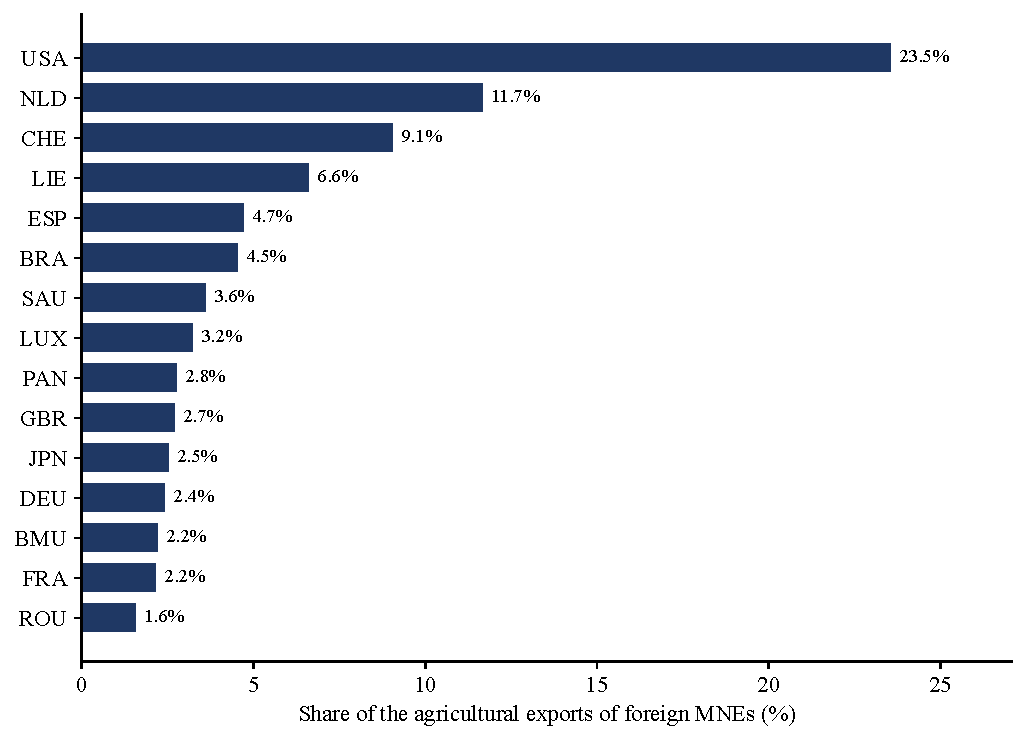
\includegraphics[width=0.78\linewidth,height=0.42\textheight,keepaspectratio]{figures/agro2018/fig_agp_parent_all.pdf}

\begin{minipage}{0.9\linewidth}
\notesize
\vspace{0.6em}
\textit{Notes:} Percent of the agricultural exports of foreign MNEs with a recorded parent country (88 percent of the total) in 2018, by country of the ultimate parent. The fifteen largest parent countries. Investment hubs (Section~\ref{sec:parents}) include Switzerland, Liechtenstein, Luxembourg, Panama, Bermuda, Hong Kong and Singapore; Appendix Table~\ref{tab:ap_panels} shows them separately.\\
\srcnote
\end{minipage}
\end{figure}

Parent countries also differ in where their affiliates sell. Affiliates of US groups send 28 percent of their
agricultural exports to Argentina, 10 percent to China and 9 percent to the United States.\footnote{Appendix Table~\ref{tab:ap_pxd18} reports the destination of the agricultural exports of foreign multinationals by parent country in 2018.} The exports to Argentina
are mostly soybeans, soybean meal and soybean oil that affiliates of large US grain traders ship from Paraguay.
Argentina took between 4 and 8 percent of the agricultural exports of foreign affiliates in each year of 2012--2017
and 11 percent in 2018, when it imported far more soybeans from Paraguay than before \citep{trase2020}. Swiss and
Liechtenstein groups sell mostly outside the ten largest destinations. Seen from the destinations, US groups supply 59 percent of the agricultural exports of foreign
affiliates that go to Argentina, 35 percent of those to Vietnam and 22 percent of those to China (Table~\ref{tab:pxd}).
Spanish groups supply 29 percent of those that go to Spain. Over 2012--2018, 4.5 percent of the agricultural exports of foreign affiliates went to the country of their parent.\footnote{Appendix Table~\ref{tab:ap_pres} reports this share by exporting country and Appendix Figure~\ref{fig:ap_home} by parent country.}

% ---- Table: Foreign-multinational agricultural exports: top 10 destinations and top 10 parents, 2018
\begin{table}[htbp]
\centering
\caption{Foreign-multinational agricultural exports: top 10 destinations and top 10 parents, 2018}
\label{tab:pxd}
{\footnotesize\setlength{\tabcolsep}{3pt}\setlength{\extrarowheight}{1pt}
\input{tables/agro2018/tab_wp1c_country_colpct_fx2}}

\begin{minipage}{0.95\linewidth}
\notesize
\vspace{0.6em}
\textit{Notes:} Percent of the agricultural exports of foreign MNEs with a recorded parent country going to each destination in 2018, by parent country (columns add to 100). Columns: the ten largest destinations of foreign-MNE exports and all other destinations. Rows: the ten largest parent countries and all other parents. The ten largest parent countries and the ten largest destinations account for 72 and 59 percent of the agricultural exports of foreign MNEs with a recorded parent country.\\
\srcnote
\end{minipage}
\end{table}

\FloatBarrier
\subsection{Fact 3: A few large groups ship most foreign-affiliate exports}

Most of the exports of foreign affiliates come from groups with large networks (Figure~\ref{fig:network}). In
2018, 41 percent of parents had only one affiliate in the world, but the 15 percent with more than 100 affiliates
shipped 49 percent of the exports of foreign affiliates. Groups with 11 to 100 affiliates shipped another 30 percent,
so groups with more than ten affiliates account for 79 percent of the total. This concentration is consistent with
large networks giving groups buyers, logistics and information in many countries at once.

% ---- Figure: Foreign-multinational agricultural exports and number of parents, by size of the group's global network, 2018
\begin{figure}[htbp]
\centering
\caption{Foreign-multinational agricultural exports and number of parents, by size of the group's global network, 2018}
\label{fig:network}
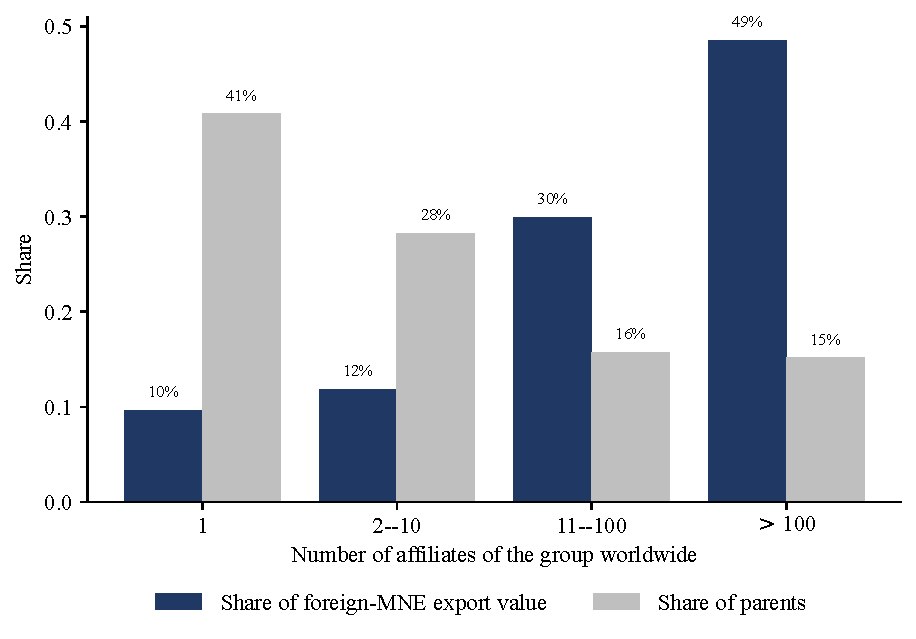
\includegraphics[width=0.78\linewidth,height=0.42\textheight,keepaspectratio]{figures/agro2018/fig_wp0_fig5_network.pdf}

\begin{minipage}{0.9\linewidth}
\notesize
\vspace{0.6em}
\textit{Notes:} Shares of foreign-MNE agricultural export value and of parents in 2018, by the number of affiliates the group has worldwide.\\
\srcnote
\end{minipage}
\end{figure}

\FloatBarrier
\subsection{Fact 4: Exports are larger where more multinationals are present}\label{sec:perf}

Exports could be larger where multinational firms are present: their affiliates bring buyers, distribution
networks and knowledge of foreign standards, and other firms can learn from them, use the same logistics or supply
them. We estimate a regression at the origin country ($o$), destination country ($d$), product ($p$) and year ($y$)
level:
\begin{equation}\label{eq:presence}
\ln X_{odpy} = \beta \ln N_{odpy} + \delta_{odp} + \delta_{ody} + \varepsilon_{odpy},
\end{equation}
where $X_{odpy}$ is the value of product $p$ exported from country $o$ to country $d$ in year $y$, and
$N_{odpy}$ is the number of multinational firms that export it. Columns 1 to 3 use the observations with at least
one multinational firm; columns 4 to 6 replace $\ln N_{odpy}$ with an indicator for at least one multinational. The
first column of each set includes origin--destination--product and year fixed effects. The second replaces the year
fixed effects with origin--destination--year fixed effects, as in equation~(\ref{eq:presence}). $\delta_{odp}$ and
$\delta_{ody}$ absorb, for example, the trade of some countries in some products to some markets every year and the
changes over time in the trade costs between two countries. The third, the strictest, adds origin--product--year and
destination--product--year fixed effects, which remove the demand for each product in each destination and year.
Standard errors are clustered by origin--destination pair.

The dependent variable is total exports in Panel A, which include the multinationals' own exports and therefore rise mechanically with their number, and the exports of local firms in Panel B. A positive Panel B coefficient is consistent with links through buyer information,
logistics or supplier relations \citep{aitken1997,mayneris2015,carballo2021}. The regression describes correlations; it does not separate the
effect of multinational firms from their choice of where to operate.

Exports are larger where more multinational firms are present, and so are the exports of local firms
(Table~\ref{tab:t1}). With origin--destination--product and origin--destination--year fixed effects, a 10 percent
higher number of multinationals is associated with about 8 percent higher exports, and at least one multinational
with exports about 90 percent higher (columns 2 and 5). With year instead of origin--destination--year fixed
effects, the estimates are similar, 0.83 and 0.66 (columns 1 and 4). For local firms, the elasticity is 0.37, and
their exports are 27 percent higher when at least one multinational is present (Panel B). The strictest
specification uses fewer observations, because each observation must share all four fixed effects with others; the
association is smaller there but still positive and significant (columns 3 and 6). The elasticity is 0.54 for total
exports and 0.16 for local firms, and at least one multinational is associated with exports 76 percent higher, and
with exports of local firms 11 percent higher.\footnote{Appendix Table~\ref{tab:ap_counts} splits multinationals by type. With origin--destination--product and origin--destination--year fixed effects, a 10 percent higher number of foreign affiliates is associated with about 4.6 percent higher exports, against 2.4 percent for domestic affiliates (column 4); for local firms, the elasticities are 0.34 and 0.24 (Appendix Table~\ref{tab:ap_counts_local}).}\textsuperscript{,}\footnote{By destination, with origin--destination--product and origin--destination--year fixed effects (column 6), the elasticity is 0.37 for other destinations and 0.24 for the parent's country, and 0.49 against 0.35 for local firms, in line with export-platform investment \citep{ekholm2007} and little intra-group trade \citep{ramondo2016}; 4.5 percent of foreign-affiliate exports go to the parent's country (Appendix Table~\ref{tab:ap_pres}).}

% ---- Table: Multinational presence and agricultural exports
\begin{table}[htbp]
\centering
\caption{Multinational presence and agricultural exports}
\label{tab:t1}
{\footnotesize\setlength{\tabcolsep}{4pt}\setlength{\extrarowheight}{1pt}
\input{tables/agro/reg_agp_presence_fx2}}

\begin{minipage}{0.95\linewidth}
\notesize
\vspace{0.6em}
\textit{Notes:} Regression at the origin country, destination country, product and year level; agricultural products, 2012--2018. Dependent variable: $\ln$ exports (Panel A) and $\ln$ exports of non-MNE firms (Panel B). Columns 1--3: $\ln$ number of MNEs, observations with at least one MNE. Columns 4--6: indicator for at least one MNE. Panel B uses only the exports of non-MNE firms, so that the exports of the multinationals themselves do not enter the dependent variable. Standard errors clustered by origin--destination pair in parentheses. *** $p<0.01$, ** $p<0.05$, * $p<0.1$.\\
\srcnote
\end{minipage}
\end{table}

\FloatBarrier
\subsection{Fact 5: The association is stronger for field crops}

Field crops, such as cereals, oilseeds, pulses and sugar crops, are grown on large areas and harvested by
machine; fruit, vegetables, coffee, cocoa, flowers and tobacco need more labor at harvest. In the United
States, labor accounts for 30 to 40 percent of the cash expenses of growers of fruit, vegetables, tree nuts and
horticultural crops \citep{kandel2008}. Products are grouped into four types of production, following the crop groups
of the FAO Indicative Crop Classification: field crops; horticultural and plantation crops; livestock and fisheries;
and other processed food and beverages.\footnote{Appendix Table~\ref{tab:ap_crop} gives the full definitions of the four types of production, with their agricultural exports and multinational shares.} Multinational firms ship 51 percent of the exports of field crops
and 40 percent of those of horticultural and plantation crops.

The specification interacts $\ln N_{odpy}$ in equation~(\ref{eq:presence}), or the indicator for at least one multinational
(columns 3 and 4), with an indicator for each type of production. Columns 1 and 3 use origin--destination--product and
origin--destination--year fixed effects, and columns 2 and 4 the strictest specification.

The association is stronger for field crops (Table~\ref{tab:crop}).
With origin--destination--product and origin--destination--year fixed effects, a 10 percent higher number of
multinationals is associated with 6.7 percent higher exports of horticultural and plantation crops and 10.0 percent
higher exports of field crops (Table~\ref{tab:crop}, column 1). The difference, 0.33, is significant at the 1 percent level. In
the strictest specification the difference is larger, 0.97 against 0.47, and also significant at the 1 percent
level (column 2). For local firms, the elasticity is 0.32 in horticultural crops and 0.53 in field crops, and at
least one multinational is associated with exports 23 and 47 percent higher (Table~\ref{tab:crop_local}, columns 1 and 3). These
differences for local firms, and the difference in the indicator specification for total exports, are not
significant in the strictest specification (columns 2 and 4). Livestock and fisheries are in between, with
elasticities of 0.92 for total exports and 0.51 for local firms (column 1); other processed food is close to
horticultural crops for total exports and lower for local firms (0.15). This is consistent with the storage,
crushing and shipping facilities that large traders operate for field crops.

Within the same origin, destination and year, the multinational share of field crops equals that of
horticultural crops, and is 4.7 percentage points higher when weighted by export value, significant only at the 10
percent level. It is 4 percentage points higher for livestock and fisheries and 8 percentage points higher
for other processed food, so the aggregate gap between field and horticultural crops comes mostly from the largest
flows.\footnote{Appendix Table~\ref{tab:ap_crop_share} reports these regressions of the multinational share on the type of production.}

% ---- Table: Multinational presence and agricultural exports, by type of production, all firms
\begin{table}[htbp]
\centering
\caption{Multinational presence and agricultural exports, by type of production, all firms}
\label{tab:crop}
{\footnotesize\setlength{\tabcolsep}{4pt}\setlength{\extrarowheight}{1pt}
\input{tables/agro/reg_agp_croptype_a_fx2}}

\begin{minipage}{0.95\linewidth}
\notesize
\vspace{0.6em}
\textit{Notes:} Regression at the origin country, destination country, product and year level; agricultural products, 2012--2018. Dependent variable: $\ln$ exports. Each coefficient is the interaction of $\ln$ number of MNEs (columns 1--2) or of the indicator for at least one MNE (columns 3--4) with an indicator for the type of production; the type of production on its own is absorbed by the origin--destination--product fixed effects. Types of production as defined in Table~\ref{tab:ap_crop}. Columns 1--2: observations with at least one MNE. Standard errors clustered by origin--destination pair in parentheses. *** $p<0.01$, ** $p<0.05$, * $p<0.1$.\\
\textit{Source:} Authors' calculations based on customs data matched to Orbis (Bureau van Dijk) and Dun \& Bradstreet; crop groups from the FAO Indicative Crop Classification.
\end{minipage}
\end{table}

% ---- Table: Multinational presence and agricultural exports, by type of production, local firms
\begin{table}[htbp]
\centering
\caption{Multinational presence and agricultural exports, by type of production, local firms}
\label{tab:crop_local}
{\footnotesize\setlength{\tabcolsep}{4pt}\setlength{\extrarowheight}{1pt}
\input{tables/agro/reg_agp_croptype_b_fx2}}

\begin{minipage}{0.95\linewidth}
\notesize
\vspace{0.6em}
\textit{Notes:} Regression and specifications as in Table~\ref{tab:crop}. Dependent variable: $\ln$ exports of non-MNE firms. Standard errors clustered by origin--destination pair in parentheses. *** $p<0.01$, ** $p<0.05$, * $p<0.1$.\\
\textit{Source:} Authors' calculations based on customs data matched to Orbis (Bureau van Dijk) and Dun \& Bradstreet; crop groups from the FAO Indicative Crop Classification.
\end{minipage}
\end{table}

\FloatBarrier
\subsection{Fact 6: The distance elasticity of exports is smaller for multinationals}

Trade falls with distance \citep{head2014}; part of the cost is fixed \citep{chaney2008} and search costs
rise with distance \citep{rauch1999}. Multinational affiliates may face lower costs through the headquarters and the
other affiliates of the group, which already know buyers in many markets. We estimate, at the firm ($f$),
destination ($d$), product ($p$) and year ($y$) level, whether the exports of multinationals fall less with distance
than those of local firms:
\begin{equation}\label{eq:dist}
\ln x_{fodpy} = \alpha \ln D_{od} + \gamma \left(M_{f} \times \ln D_{od}\right) + \delta_{oy} + \delta_{dy} + \delta_{p} + u_{fodpy},
\end{equation}
where $x_{fodpy}$ is the value of product $p$ exported by firm $f$, located in $o$, to $d$ in year $y$. $D_{od}$
is the distance between the two countries, from the CEPII gravity database, and $M_f$ equals one for a multinational
affiliate. The coefficient $\alpha$ is the distance elasticity of local firms and $\gamma$ the difference for
multinational affiliates. The fixed effects absorb origin and destination shocks in each year and product
differences; other columns use origin, destination and year fixed effects. Columns 3 and 4 split affiliates by
whether the group is present in the destination. Standard errors are clustered by origin--destination pair, and the
regression describes correlations.

The distance elasticity of exports is smaller for multinational affiliates than for local firms
(Table~\ref{tab:t2}). The exports of local firms fall by about 0.21 to 0.22 percent for each 1 percent of distance.
The elasticity is about 15 percent smaller for multinational affiliates, and about 40 percent smaller when the group
has an affiliate in the destination or the destination is the parent's country (columns 3 and 4). The larger gap
where the group is present is consistent with lower costs of reaching markets where the group already
operates.\footnote{Appendix Table~\ref{tab:ap_dist} separates foreign and domestic affiliates. The elasticity is about 17 percent smaller for foreign affiliates (interaction 0.038, base elasticity $-0.21$) and about 9 percent smaller for domestic ones (0.020) (columns 1 and 2); among foreign affiliates, the gap is larger for exports to the parent's country (0.065) than to other countries (0.037) (columns 3 and 4).}

% ---- Table: Distance and firm agricultural exports: multinationals by presence at the destination
\begin{table}[htbp]
\centering
\caption{Distance and firm agricultural exports: multinationals by presence at the destination}
\label{tab:t2}
{\footnotesize\setlength{\tabcolsep}{4pt}\setlength{\extrarowheight}{1pt}
\input{tables/agro/reg_agp_distance_early_fx2}}

\begin{minipage}{0.95\linewidth}
\notesize
\vspace{0.6em}
\textit{Notes:} Regression at the firm, destination country, product and year level; agricultural products, 2012--2018. Dependent variable: $\ln$ exports. Local (non-MNE) firms are the omitted group. Columns 1--2: all MNEs; columns 3--4: MNEs split by whether the group is present at the destination. Present: the group has an affiliate in the destination or the destination is the parent's country. The MNE indicators enter only through their interactions with distance. Standard errors clustered by origin--destination pair in parentheses. *** $p<0.01$, ** $p<0.05$, * $p<0.1$.\\
\textit{Source:} Authors' calculations based on customs data matched to Orbis (Bureau van Dijk) and Dun \& Bradstreet; distances from the CEPII gravity database.
\end{minipage}
\end{table}

%======================================================================
\section{Conclusion}\label{sec:concl}
%======================================================================
Matched customs and ownership data for nine Latin American countries show that multinational firms ship almost
half of the region's agricultural exports: 40 percent through foreign affiliates and 8 percent through domestic ones
in 2018. The share stayed between 47 and 50 percent every year of 2012--2018. Multinational affiliates are a quarter of agricultural
exporters, but they export between two and three times as much as local firms and reach more markets.

Ownership is concentrated. A few parent countries, led by the United States and the Netherlands, and a few
groups with more than 100 affiliates account for most foreign-affiliate exports. Exports, including those
of local firms, are larger where more multinational firms are present, especially for field crops. The distance elasticity of exports is smaller for multinational affiliates than for local firms, and smaller still when the group is present in the destination.

Considering that they describe correlations, the results suggest three policy implications. Policies that
attract foreign investment, such as investment promotion \citep{harding2011,volpe2021,carballo2026}, are also export policies. Supplier links to multinationals
\citep{alfarourena2022,carballo2021} and export promotion \citep{volpe2008} could extend the reach of local firms, which ship half of agricultural exports. Governments need
better information on who owns their exporters, given the weight of a few groups and of parents recorded in investment hubs.

\clearpage
\bibliographystyle{elsarticle-harv}
\bibliography{Note_refs}

\clearpage
\appendix
\setcounter{figure}{0}\renewcommand{\thefigure}{A.\arabic{figure}}
\setcounter{table}{0}\renewcommand{\thetable}{A.\arabic{table}}
\renewcommand{\thesubsection}{A.\arabic{subsection}}
\section*{Appendix}\label{sec:app}

This appendix reports descriptive statistics and additional estimates for the agricultural exports of the nine countries, from customs records matched to Orbis and Dun \& Bradstreet. The exhibits cover 2012--2018 unless the caption says 2018; their notes state whether values are annual averages, pooled shares or yearly figures. Exporters are classified as in Section~\ref{sec:data}.

\subsection{Descriptive statistics}
Tables~\ref{tab:ap_summary}, \ref{tab:ap_sample} and~\ref{tab:ap_desttab} report the sample summary, agricultural exports by exporting country, and agricultural exports and ownership by destination region, as annual averages over 2012--2018.
% ---- Table: Agricultural sample summary, annual averages 2012--2018
\begin{table}[htbp]
\centering
\caption{Agricultural sample summary, annual averages 2012--2018}
\label{tab:ap_summary}
{\small\setlength{\tabcolsep}{4pt}\setlength{\extrarowheight}{1pt}
\input{tables/agro/tab_agp_summary_fx3}}

\begin{minipage}{0.95\linewidth}
\notesize
\vspace{0.6em}
\textit{Notes:} Agricultural exports of the nine countries, 2012--2018. Exports per year are annual averages; shares by type of exporter are percent of agricultural export value. Exporting firms per year: average number of exporting firms in a year, summed over countries. Destination countries are counted as in Table~\ref{tab:summary}.\\
\srcnote
\end{minipage}
\end{table}
% ---- Table: Agricultural exports, by exporting country, annual averages 2012--2018
\begin{table}[htbp]
\centering
\caption{Agricultural exports, by exporting country, annual averages 2012--2018}
\label{tab:ap_sample}
{\footnotesize\setlength{\tabcolsep}{3pt}\setlength{\extrarowheight}{1pt}
\input{tables/agro/tab_agp_sample_fx3}}

\begin{minipage}{0.95\linewidth}
\notesize
\vspace{0.6em}
\textit{Notes:} Agricultural exports (HS 01--24), 2012--2018. Exporters are distinct tax identifiers within each country; MNE affiliates are exporters linked to Orbis or Dun \& Bradstreet. Exports are annual averages in US\$ billion. Agriculture in total exports: percent of the country's merchandise exports. MNE share: percent of the country's agricultural exports shipped by MNE affiliates.\\
\srcnote
\end{minipage}
\end{table}
% ---- Table: Agricultural exports and ownership, by destination region, annual averages 2012--2018
\begin{table}[htbp]
\centering
\caption{Agricultural exports and ownership, by destination region, annual averages 2012--2018}
\label{tab:ap_desttab}
{\small\setlength{\tabcolsep}{4pt}\setlength{\extrarowheight}{1pt}
\input{tables/agro/tab_agp_dest_fx2}}

\begin{minipage}{0.95\linewidth}
\notesize
\vspace{0.6em}
\textit{Notes:} Column (1): percent of the agricultural exports of the nine countries going to each region. Columns (2)--(4): percent of the exports to each region shipped by each type of exporter. Exports are annual averages over 2012--2018, in US\$ billion.\\
\srcnote
\end{minipage}
\end{table}

Agricultural exports followed commodity prices, while the role of multinational firms remained stable
(Table~\ref{tab:ap_trend}). The exports of the nine countries peaked at US\$82.5 billion in 2013, fell to US\$73.6
billion in 2015 and recovered to US\$78.5 billion in 2018. Multinational firms shipped between 47 and 50 percent of
the total in every year, and foreign affiliates alone between 37 and 41 percent. The share is also stable within most
countries (Table~\ref{tab:ap_cy}). It changed by less than five percentage points in six of the nine countries; it
rose from 57 to 72 percent in Uruguay and from 63 to 69 percent in Paraguay, and fell from 51 to 45 percent in the
Dominican Republic.
% ---- Table: Agricultural exports by type of exporter, 2012--2018
\begin{table}[htbp]
\centering
\caption{Agricultural exports by type of exporter, 2012--2018}
\label{tab:ap_trend}
{\small\setlength{\tabcolsep}{4pt}\setlength{\extrarowheight}{1pt}
\input{tables/agro/tab_agp_trend_fx}}

\begin{minipage}{0.95\linewidth}
\notesize
\vspace{0.6em}
\textit{Notes:} Agricultural exports of the nine countries, in current US\$ billion, and percent shipped by each type of exporter.\\
\srcnote
\end{minipage}
\end{table}
% ---- Table: Multinational share of agricultural exports, by exporting country and year
\begin{table}[htbp]
\centering
\caption{Multinational share of agricultural exports, by exporting country and year}
\label{tab:ap_cy}
{\footnotesize\setlength{\tabcolsep}{4pt}\setlength{\extrarowheight}{1pt}
\input{tables/agro/tab_agp_country_year_fx2}}

\begin{minipage}{0.95\linewidth}
\notesize
\vspace{0.6em}
\textit{Notes:} Percent of each country's agricultural exports shipped by MNE affiliates (foreign and domestic), 2012--2018. LAC9: the nine countries together.\\
\srcnote
\end{minipage}
\end{table}

The geography of these exports changed more than their ownership (Table~\ref{tab:dest}). In 2018, Latin America
and the Caribbean took 26 percent of the exports, Europe 24 percent, Asia without China 18 percent, the United States
and Canada 16 percent, China 10 percent and Africa 6 percent. Between 2012 and 2018, the share of other Latin American
countries fell from 29 to 26 percent, while that of the United States and Canada rose from 13 to 16 percent and that
of China from 9 to 10 percent (Table~\ref{tab:ap_trend_dest}). Foreign affiliates ship 51 percent of the exports to
other Latin American countries and 44 percent of those to China, against 34 percent of those to Europe and to the
United States and Canada.
% ---- Table: Agricultural exports and ownership, by destination region, 2018
\begin{table}[htbp]
\centering
\caption{Agricultural exports and ownership, by destination region, 2018}
\label{tab:dest}
{\small\setlength{\tabcolsep}{4pt}\setlength{\extrarowheight}{1pt}
\input{tables/agro2018/tab_agp_dest_fx2}}

\begin{minipage}{0.95\linewidth}
\notesize
\vspace{0.6em}
\textit{Notes:} Column (1): percent of the agricultural exports of the nine countries going to each region in 2018. Columns (2)--(4): percent of the exports to each region shipped by each type of exporter. Exports in US\$ billion. China includes Hong Kong and Macao.\\
\srcnote
\end{minipage}
\end{table}
% ---- Table: Destination of agricultural exports, 2012--2018
\begin{table}[htbp]
\centering
\caption{Destination of agricultural exports, 2012--2018}
\label{tab:ap_trend_dest}
{\footnotesize\setlength{\tabcolsep}{3pt}\setlength{\extrarowheight}{1pt}
\input{tables/agro/tab_agp_trend_dest_fx2}}

\begin{minipage}{0.95\linewidth}
\notesize
\vspace{0.6em}
\textit{Notes:} Percent of the agricultural exports of the nine countries going to each destination region (rows add to 100). Latin America includes the Caribbean.\\
\srcnote
\end{minipage}
\end{table}

Multinational affiliates are a quarter of agricultural exporters, but they are larger and sell to more markets
than local firms (Table~\ref{tab:ap_firms}). In 2018, foreign affiliates were 20 percent of exporters and shipped 40
percent of the value, while local firms were 76 percent of exporters and shipped 52 percent. A foreign affiliate
exported on average US\$12.0 million and a domestic affiliate US\$10.5 million, between two and three times as much
as a local firm (US\$4.2 million). Affiliates also reach more destinations, 5.5 for foreign and 6.1 for domestic
affiliates on average against 3.9 for local firms; the number of products per firm is similar in the three groups.
% ---- Table: Agricultural exporters, by type of owner, 2018
\begin{table}[htbp]
\centering
\caption{Agricultural exporters, by type of owner, 2018}
\label{tab:ap_firms}
{\small\setlength{\tabcolsep}{4pt}\setlength{\extrarowheight}{1pt}
\input{tables/agro2018/tab_agp_firms_fx}}

\begin{minipage}{0.95\linewidth}
\notesize
\vspace{0.6em}
\textit{Notes:} Agricultural exporters of the nine countries in 2018. Exporters are distinct tax identifiers within each country. Exports, products and destinations are computed for each firm and then averaged over firms.\\
\srcnote
\end{minipage}
\end{table}

The products are concentrated in a few groups (Table~\ref{tab:ap_sitc} and Figure~\ref{fig:ap_hs6}). Over
2012--2018, animal feed (US\$14.1 billion a year, mostly soybean meal), vegetables and fruit (10.4), cereals (10.3),
oil seeds (7.1) and vegetable oils (5.8) were the largest, and soybean meal, soybeans and crude soybean oil alone
amounted to US\$21.8 billion a year, 28 percent of the total. US groups lead in oil seeds (54 percent of the exports of foreign affiliates) and cereals (33 percent),
Swiss and Liechtenstein groups in animal feed (28 and 19 percent), German groups in coffee (42 percent), Saudi and
Brazilian groups in meat, and Spanish groups in fish and in vegetables and fruit. Agricultural inputs (seeds, animal
feed and live animals) and the remaining products have similar foreign shares, 36 and 40 percent
(Table~\ref{tab:ap_inputs}).
% ---- Table: Agricultural exports and multinational shares, by product group
\begin{table}[htbp]
\centering
\caption{Agricultural exports and multinational shares, by product group}
\label{tab:ap_sitc}
{\footnotesize\setlength{\tabcolsep}{4pt}\setlength{\extrarowheight}{1pt}
\input{tables/agro/tab_wp2_sitc2_fx2}}

\begin{minipage}{0.95\linewidth}
\notesize
\vspace{0.6em}
\textit{Notes:} Agricultural exports by SITC Rev.\,3 division, 2012--2018. Foreign and domestic: percent of the division's export value. Leading parents: the three largest parent countries and their share of the division's foreign-MNE exports. Values are annual averages over 2012--2018, in US\$ billion. Products without an SITC correspondence (US\$6.0 billion a year) are excluded.\\
\srcnote
\end{minipage}
\end{table}
% ---- Figure: Ownership of the twenty largest agricultural export products
\begin{figure}[htbp]
\centering
\caption{Ownership of the twenty largest agricultural export products}
\label{fig:ap_hs6}
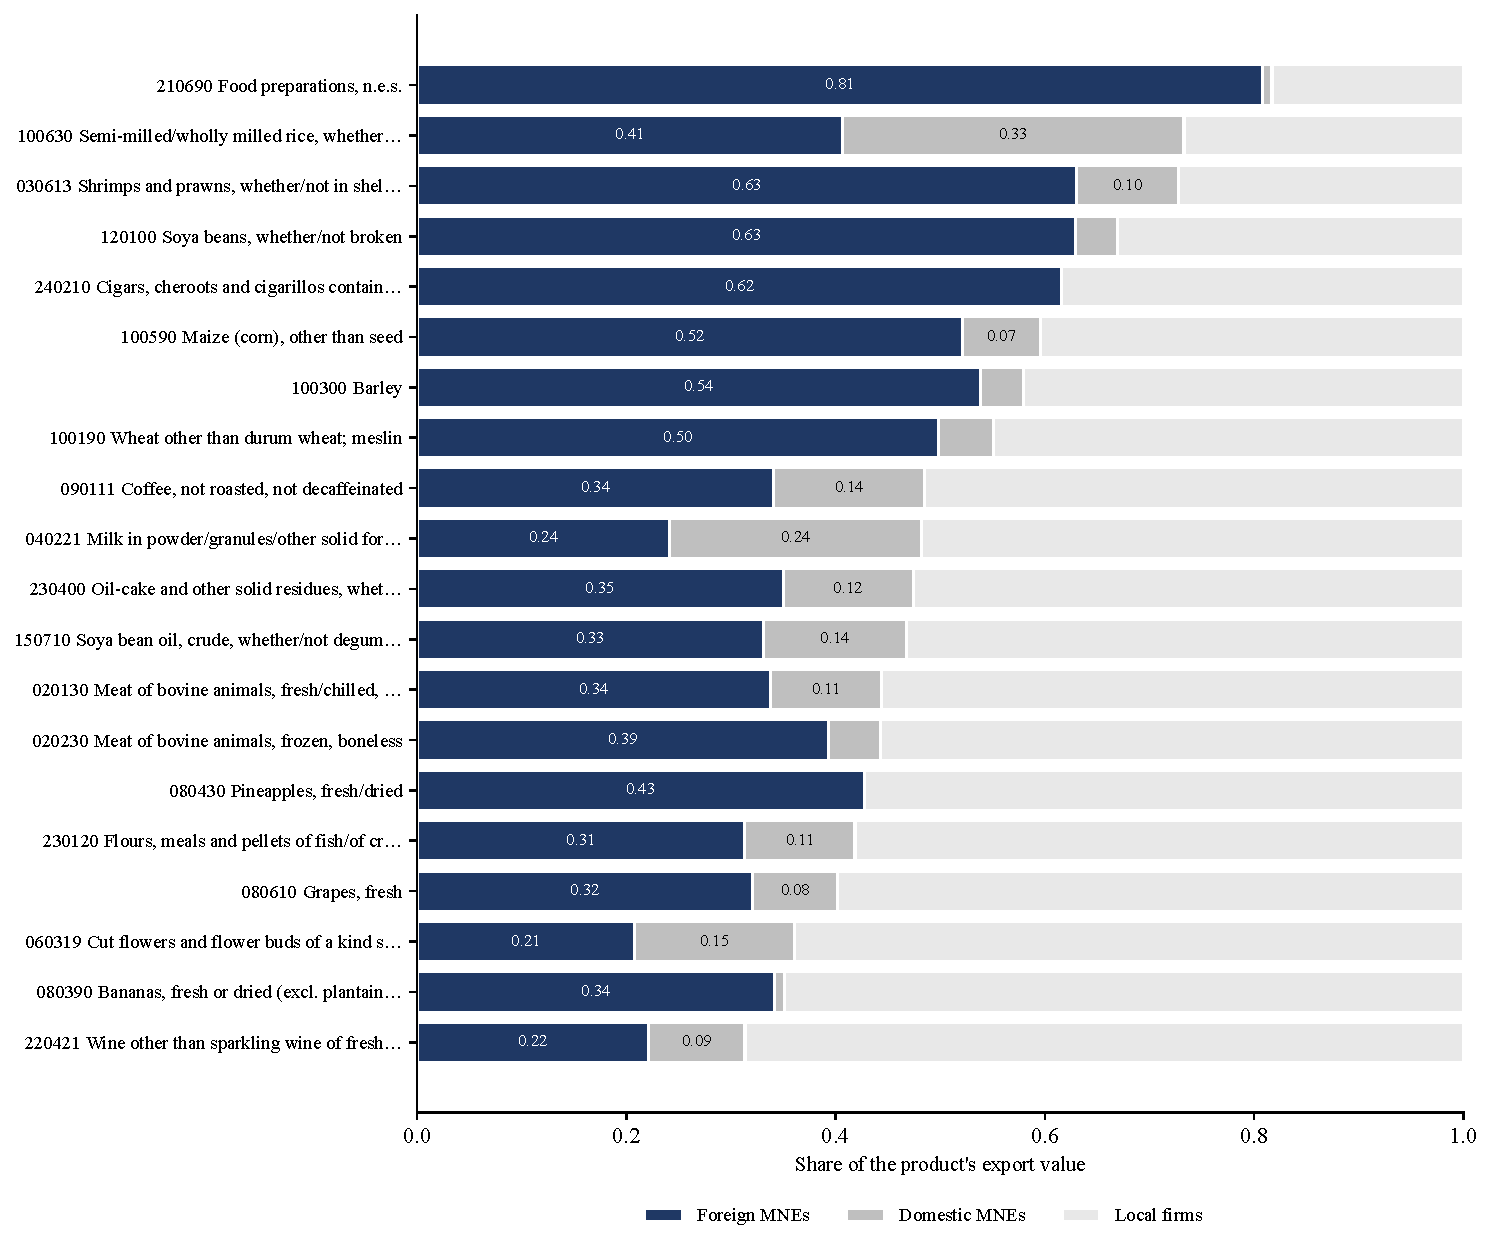
\includegraphics[width=0.78\linewidth,height=0.42\textheight,keepaspectratio]{figures/agro/fig_wp1f_top20_hs6_stacked.pdf}

\begin{minipage}{0.9\linewidth}
\notesize
\vspace{0.6em}
\textit{Notes:} Shares of each product's export value, by type of exporter, 2012--2018. The twenty largest agricultural products by export value, ordered by MNE share, largest first.\\
\srcnote
\end{minipage}
\end{figure}
% ---- Table: Agricultural exports and multinational shares: inputs and other products
\begin{table}[htbp]
\centering
\caption{Agricultural exports and multinational shares: inputs and other products}
\label{tab:ap_inputs}
{\small\setlength{\tabcolsep}{4pt}\setlength{\extrarowheight}{1pt}
\input{tables/agro/tab_wp2_inputs_fx2}}

\begin{minipage}{0.95\linewidth}
\notesize
\vspace{0.6em}
\textit{Notes:} Inputs: seeds, animal feed and live animals. Foreign and domestic: percent of the group's export value, 2012--2018. Leading parents: the three largest parent countries and their share of the group's foreign-MNE exports. Values are annual averages over 2012--2018, in US\$ billion.\\
\srcnote
\end{minipage}
\end{table}

Grouping products by type of farm production gives a similar picture (Table~\ref{tab:ap_crop}). Multinational
firms ship 51 percent of the exports of field crops (cereals, oilseeds, pulses, roots and sugar crops, with their
flour, oils and meal), which are grown on large areas and harvested by machine, and 40 percent of the exports of
horticultural and plantation crops (fruit, vegetables, coffee, cocoa, spices, flowers and tobacco), whose harvest
uses much more labor.
% ---- Table: Agricultural exports and multinational shares, by type of production
\begin{table}[htbp]
\centering
\caption{Agricultural exports and multinational shares, by type of production}
\label{tab:ap_crop}
{\small\setlength{\tabcolsep}{4pt}\setlength{\extrarowheight}{1pt}
\input{tables/agro/tab_agp_croptype_fx2}}

\begin{minipage}{0.95\linewidth}
\notesize
\vspace{0.6em}
\textit{Notes:} Agricultural exports, 2012--2018; exports are annual averages in US\$ billion. Field crops: cereals, oilseeds, pulses, roots and sugar crops (groups 1, 4, 5, 7 and 8 of the FAO Indicative Crop Classification), their milling and crushing products (flour, vegetable oils, oilcake and meal) and fodder. Horticultural and plantation crops: fruit and nuts, vegetables, coffee, tea, cocoa and spices, flowers and live plants, tobacco, hops and medicinal plants (ICC groups 2, 3, 6 and part of 9), their preparations (HS 20) and wine. Livestock and fisheries: HS 01--05 and 16, animal fats and meat or fish meal. Other processed food and beverages: the remaining products. Products are assigned by their four-digit HS heading.\\
\textit{Source:} Authors' calculations based on customs data matched to Orbis (Bureau van Dijk) and Dun \& Bradstreet; crop groups from the FAO Indicative Crop Classification.
\end{minipage}
\end{table}
% ---- Table: Multinational share of agricultural exports, by type of production: regressions
\begin{table}[htbp]
\centering
\caption{Multinational share of agricultural exports, by type of production: regressions}
\label{tab:ap_crop_share}
{\footnotesize\setlength{\tabcolsep}{4pt}\setlength{\extrarowheight}{1pt}
\input{tables/agro/reg_agp_croptype_share_fx2}}

\begin{minipage}{0.95\linewidth}
\notesize
\vspace{0.6em}
\textit{Notes:} Regression at the origin country, destination country, product and year level; agricultural products, 2012--2018. Dependent variable: share of all MNEs (Panel A) and of foreign MNEs (Panel B) in the value exported, between 0 and 1. Horticultural and plantation crops are the omitted group. Columns 3 and 4 weight each observation by its export value. Standard errors clustered by origin--destination pair in parentheses. *** $p<0.01$, ** $p<0.05$, * $p<0.1$.\\
\textit{Source:} Authors' calculations based on customs data matched to Orbis (Bureau van Dijk) and Dun \& Bradstreet; crop groups from the FAO Indicative Crop Classification.
\end{minipage}
\end{table}

\FloatBarrier
\subsection{Parent countries and destinations}
Table~\ref{tab:ap_panels} reports foreign-multinational agricultural exports by parent country over 2012--2018 and shows the investment hubs separately from the other parent countries. Table~\ref{tab:ap_pxd18} shows where the foreign affiliates of each parent country send their agricultural exports in 2018, and Figure~\ref{fig:ap_home} the share that each parent country's affiliates ship to that same country.
% ---- Table: Foreign-multinational agricultural exports, by parent country: other countries and investment hubs
\begin{table}[htbp]
\centering
\caption{Foreign-multinational agricultural exports, by parent country: other countries and investment hubs}
\label{tab:ap_panels}
{\small\setlength{\tabcolsep}{4pt}\setlength{\extrarowheight}{1pt}
\input{tables/agro/tab_agp_parent_panels_fx3}}

\begin{minipage}{0.95\linewidth}
\notesize
\vspace{0.6em}
\textit{Notes:} Percent of foreign-MNE agricultural export value with a recorded parent country, by country of the ultimate parent, 2012--2018. The two panels add to 100. Investment hubs as defined in Section~\ref{sec:parents}.\\
\srcnote
\end{minipage}
\end{table}
% ---- Table: Destination of foreign-multinational agricultural exports, by parent country, 2018
\begin{table}[htbp]
\centering
\caption{Destination of foreign-multinational agricultural exports, by parent country, 2018}
\label{tab:ap_pxd18}
{\footnotesize\setlength{\tabcolsep}{3pt}\setlength{\extrarowheight}{1pt}
\input{tables/agro2018/tab_wp1c_country_rowpct_fx2}}

\begin{minipage}{0.95\linewidth}
\notesize
\vspace{0.6em}
\textit{Notes:} Percent of the agricultural exports of foreign MNEs with a recorded parent country going to each destination in 2018 (rows add to 100). Rows: the ten largest parent countries and all other parents. Columns: the ten largest destinations and all other destinations.\\
\srcnote
\end{minipage}
\end{table}
% ---- Figure: Share of foreign-multinational agricultural exports shipped to the parent country
\begin{figure}[htbp]
\centering
\caption{Share of foreign-multinational agricultural exports shipped to the parent country}
\label{fig:ap_home}
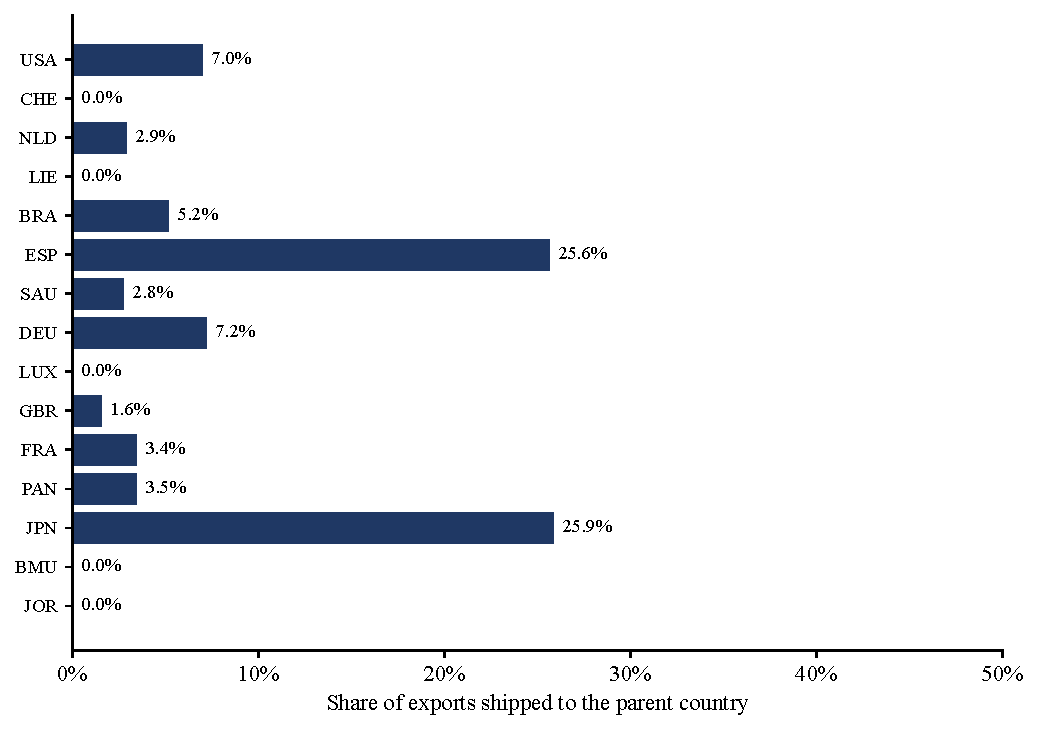
\includegraphics[width=0.78\linewidth,height=0.42\textheight,keepaspectratio]{figures/agro/fig_wp1d_home_share_by_parent.pdf}

\begin{minipage}{0.9\linewidth}
\notesize
\vspace{0.6em}
\textit{Notes:} Percent of each parent country's agricultural exports shipped to that same country, 2012--2018.\\
\srcnote
\end{minipage}
\end{figure}

\FloatBarrier
\subsection{Additional estimates}
Tables~\ref{tab:ap_counts} and~\ref{tab:ap_counts_local} estimate equation~(\ref{eq:presence}) with the number of multinational affiliates of each type and split foreign affiliates by whether the destination is the parent's country. Table~\ref{tab:ap_dist} estimates equation~(\ref{eq:dist}) with separate distance interactions for foreign and domestic affiliates, and Table~\ref{tab:ap_pres} reports the share of foreign-affiliate exports shipped to the parent's country, by exporting country.
% ---- Table: Multinational presence and agricultural exports, by type of multinational, all firms
\begin{table}[htbp]
\centering
\caption{Multinational presence and agricultural exports, by type of multinational, all firms}
\label{tab:ap_counts}
{\footnotesize\setlength{\tabcolsep}{4pt}\setlength{\extrarowheight}{1pt}
\input{tables/agro/reg_agp_counts_a_fx2}}

\begin{minipage}{0.95\linewidth}
\notesize
\vspace{0.6em}
\textit{Notes:} Regression at the origin country, destination country, product and year level; agricultural products, 2012--2018. Dependent variable: $\ln$ exports. Regressors: $\ln$ number of MNEs of each type. Columns (5)--(6) split foreign MNEs by whether the destination is the parent's country. Standard errors clustered by origin--destination pair in parentheses. *** $p<0.01$, ** $p<0.05$, * $p<0.1$.\\
\srcnote
\end{minipage}
\end{table}

% ---- Table: Multinational presence and agricultural exports, by type of multinational, local firms
\begin{table}[htbp]
\centering
\caption{Multinational presence and agricultural exports, by type of multinational, local firms}
\label{tab:ap_counts_local}
{\footnotesize\setlength{\tabcolsep}{4pt}\setlength{\extrarowheight}{1pt}
\input{tables/agro/reg_agp_counts_b_fx2}}

\begin{minipage}{0.95\linewidth}
\notesize
\vspace{0.6em}
\textit{Notes:} Regression and specifications as in Table~\ref{tab:ap_counts}. Dependent variable: $\ln$ exports of non-MNE firms, so that the exports of the multinationals themselves do not enter the dependent variable. Standard errors clustered by origin--destination pair in parentheses. *** $p<0.01$, ** $p<0.05$, * $p<0.1$.\\
\srcnote
\end{minipage}
\end{table}
% ---- Table: Distance and firm agricultural exports: foreign and domestic multinationals
\begin{table}[htbp]
\centering
\caption{Distance and firm agricultural exports: foreign and domestic multinationals}
\label{tab:ap_dist}
{\footnotesize\setlength{\tabcolsep}{4pt}\setlength{\extrarowheight}{1pt}
\input{tables/agro/reg_agp_distance_hq_fx2}}

\begin{minipage}{0.95\linewidth}
\notesize
\vspace{0.6em}
\textit{Notes:} Regression at the firm, destination country, product and year level; agricultural products, 2012--2018. Dependent variable: $\ln$ exports. Local (non-MNE) firms are the omitted group. Columns (3)--(4) split foreign MNEs by whether the destination is the parent's country. Standard errors clustered by origin--destination pair in parentheses. *** $p<0.01$, ** $p<0.05$, * $p<0.1$.\\
\textit{Source:} Authors' calculations based on customs data matched to Orbis (Bureau van Dijk) and Dun \& Bradstreet; distances from the CEPII gravity database.
\end{minipage}
\end{table}
% ---- Table: Multinational agricultural exports by exporting country and destination type
\begin{table}[htbp]
\centering
\caption{Multinational agricultural exports by exporting country and destination type}
\label{tab:ap_pres}
{\small\setlength{\tabcolsep}{3pt}\setlength{\extrarowheight}{1pt}
\input{tables/agro/tab_wp1e_presence_shares_fx3}}

\begin{minipage}{0.95\linewidth}
\notesize
\vspace{0.6em}
\textit{Notes:} MNE and foreign-MNE agricultural export value by country, and the split of foreign-MNE value by destination, 2012--2018. Parent country: exports to the country of the ultimate parent. Other: all remaining destinations; in parentheses, destinations where the group has another affiliate. Values are annual averages over 2012--2018, in US\$ billion.\\
\srcnote
\end{minipage}
\end{table}

\FloatBarrier
\end{document}
